\section{РЕЗУЛЬТАТЫ ВИЗУАЛИЗАЦИИ}
\label{sec:visualization}

\begin{figure}[h]
\centering
  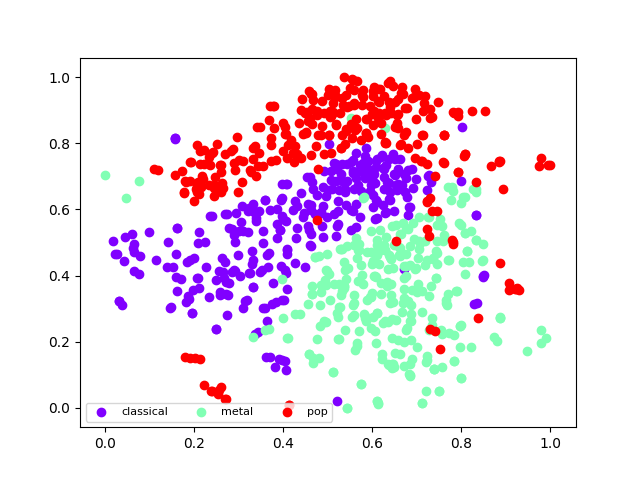
\includegraphics{vis1.png}
  \caption{Отображения пространства  признаков музыкальных треков в двухмерное простарнство алгоритмом t-SNE.}
  \label{fig:results:2dtsne}
\end{figure}

\begin{figure}[h]
\centering
  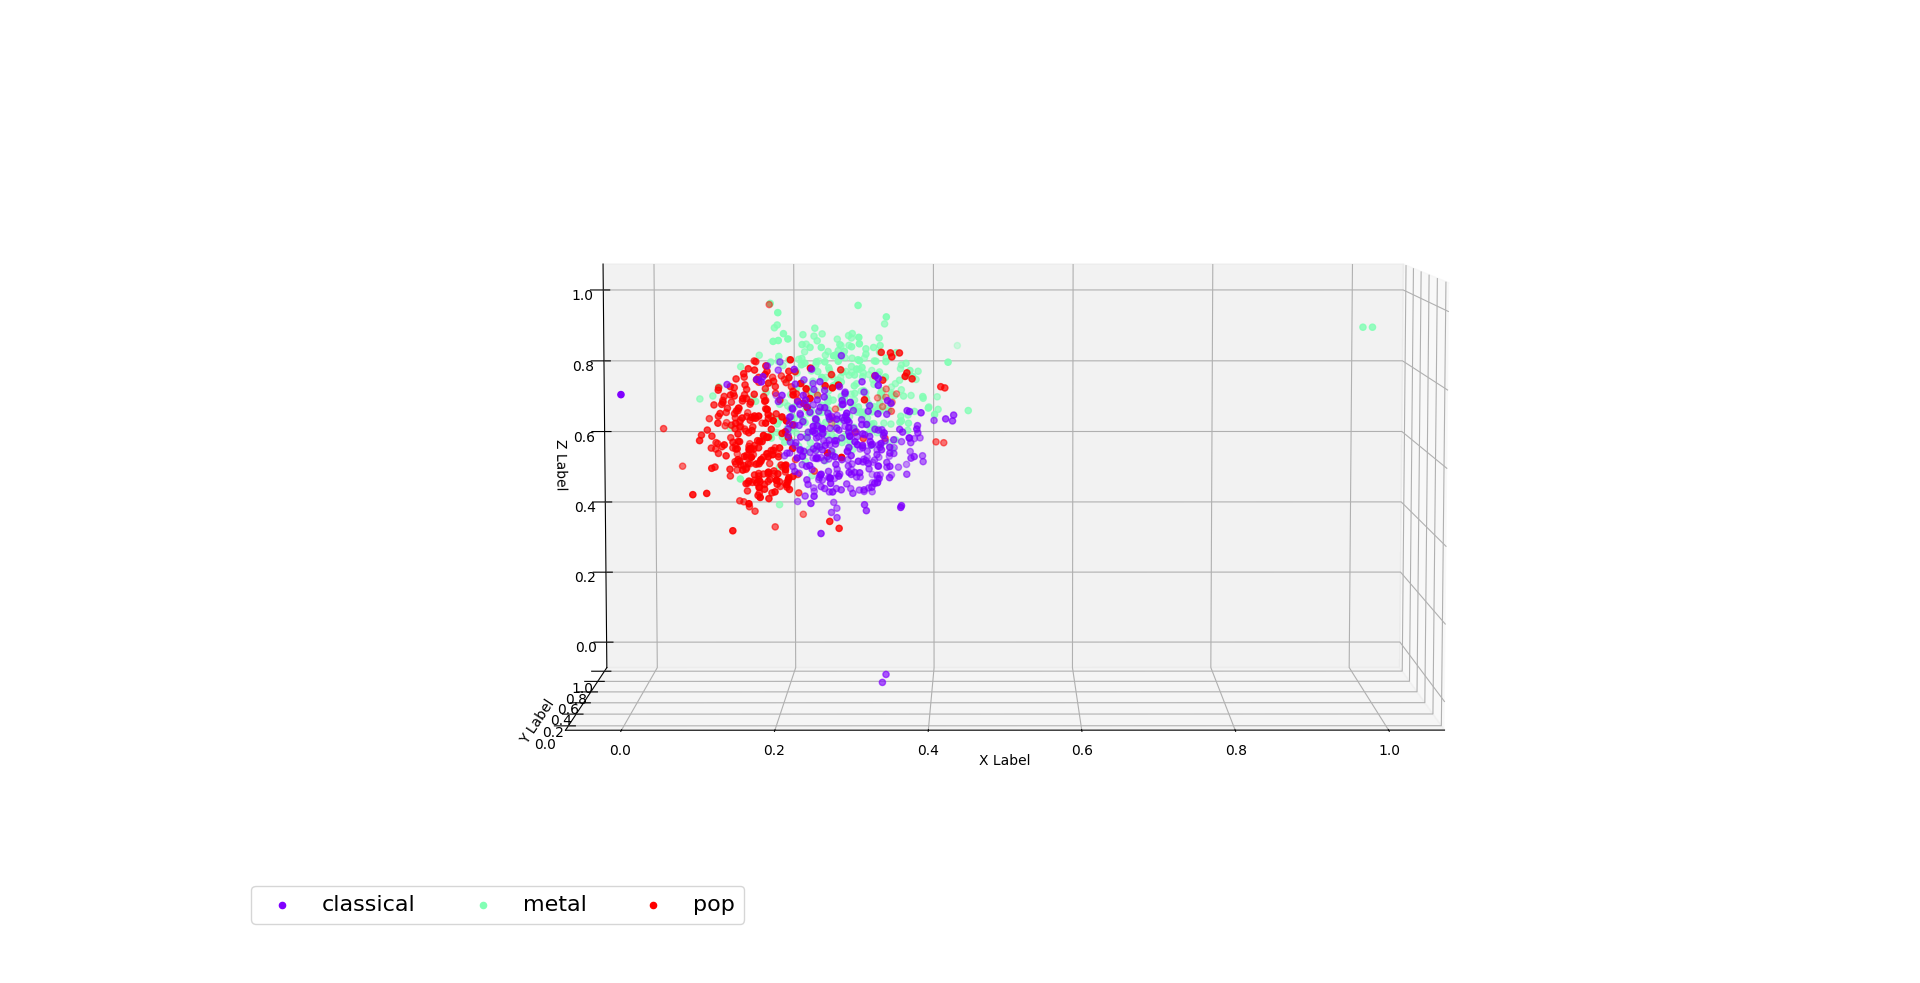
\includegraphics{3dtsne1.png}
  \caption{Отображения пространства  признаков музыкальных треков в трёхмерное пространство алгоритмом t-SNE. Первая проекция. }
  \label{fig:results:2dtsne}
\end{figure}


\begin{figure}[h]
\centering
  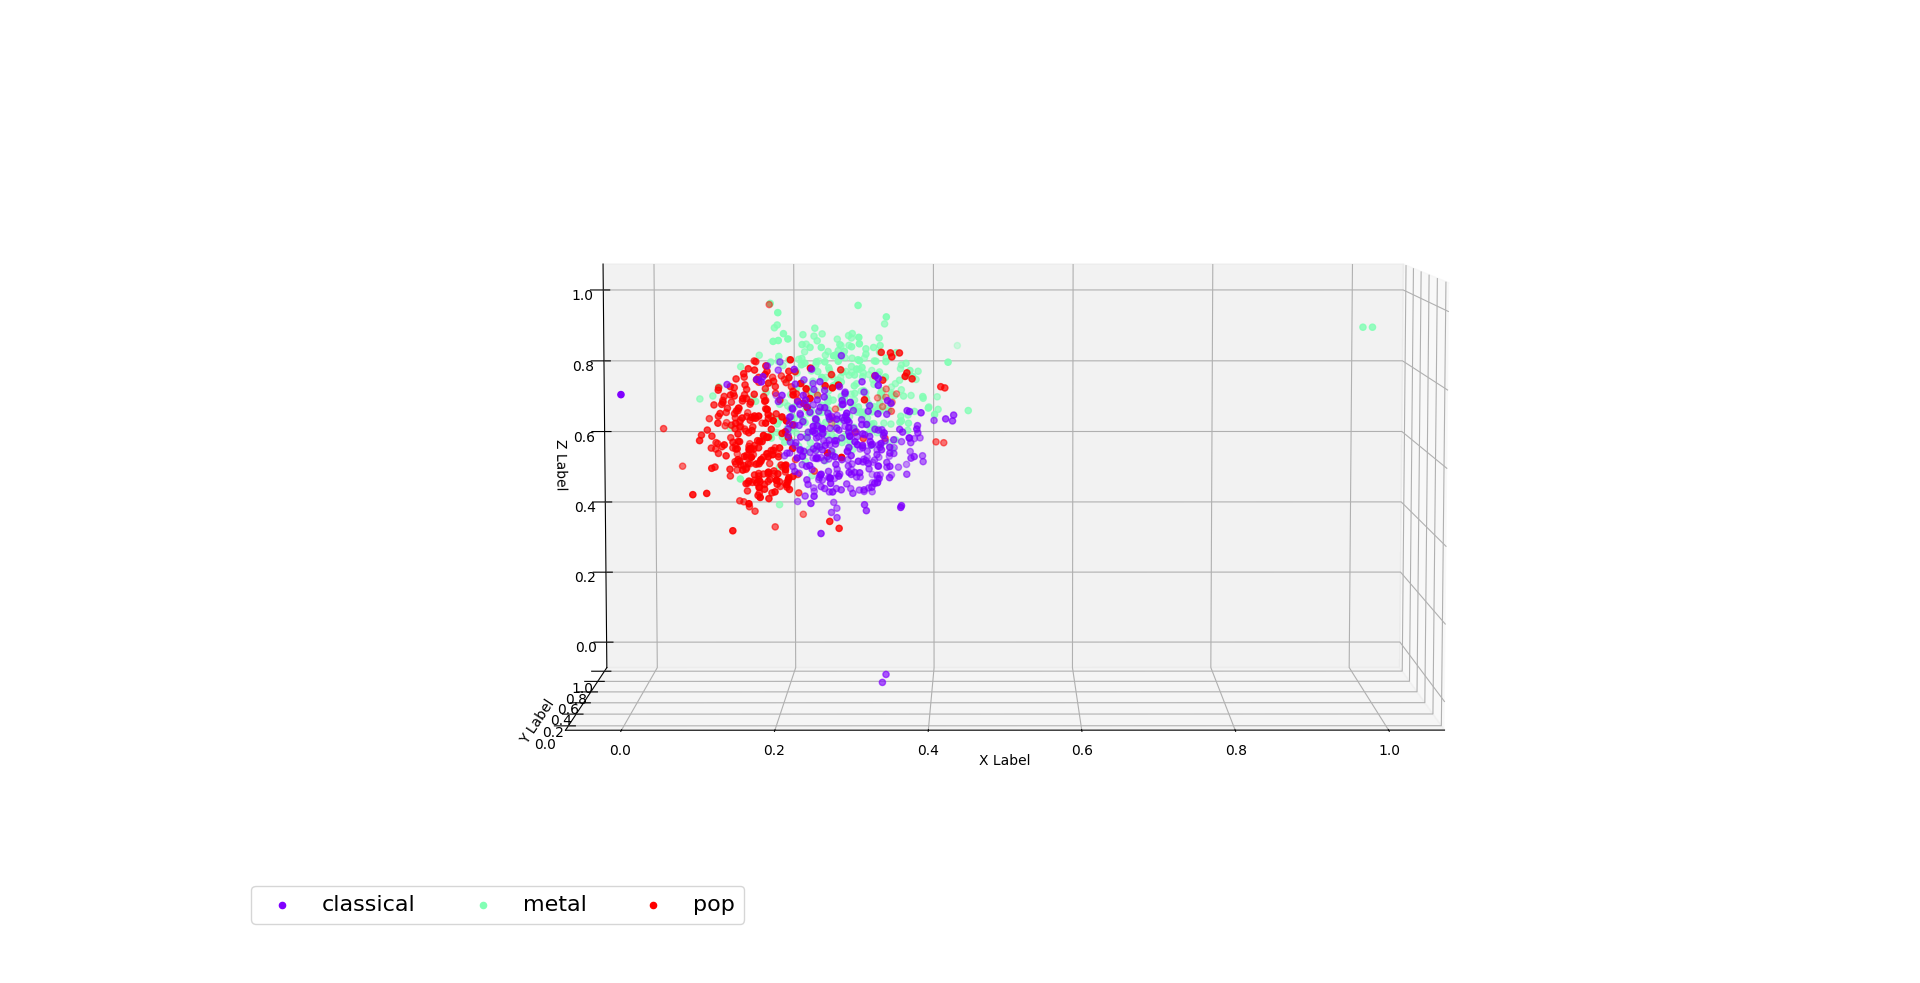
\includegraphics{3dtsne1.png}
  \caption{Отображения пространства  признаков музыкальных треков в трёхмерное пространство алгоритмом t-SNE. Вторая проекция. }
  \label{fig:results:2dtsne}
\end{figure}


\begin{figure}[h]
\centering
  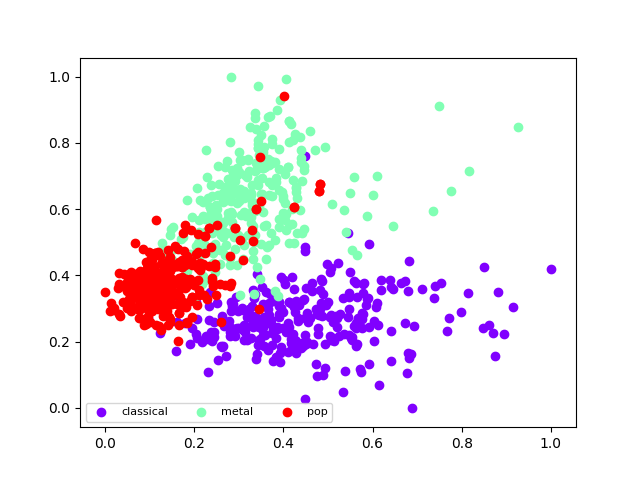
\includegraphics{2dpca.png}
  \caption{Отображения пространства  признаков музыкальных треков в двухмерное простарнство алгоритмом PCA.}
  \label{fig:results:2dtsne}
\end{figure}

\begin{figure}[h]
\centering
  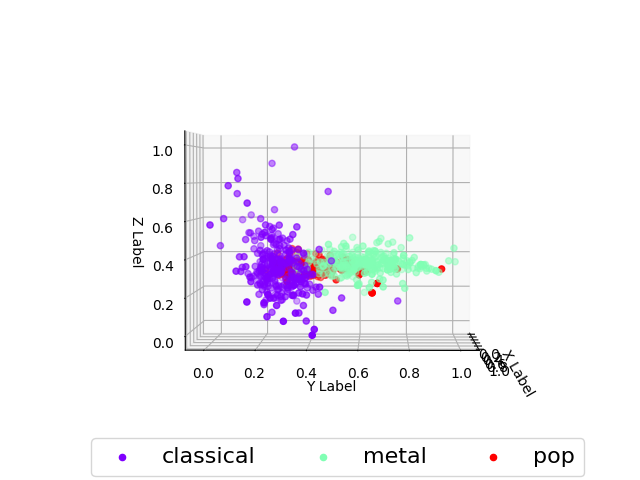
\includegraphics{3dpca1.png}
  \caption{Отображения пространства  признаков музыкальных треков в трёхмерное пространство алгоритмом PCA. Первая проекция. }
  \label{fig:results:2dtsne}
\end{figure}


\begin{figure}[h]
\centering
  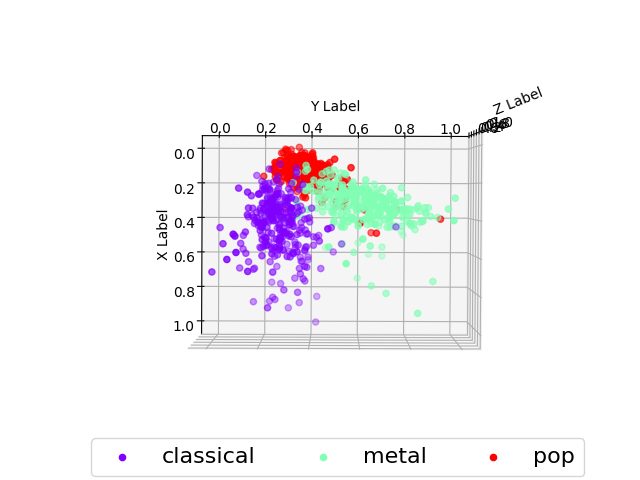
\includegraphics{3dpca2.png}
  \caption{Отображения пространства  признаков музыкальных треков в трёхмерное пространство алгоритмом PCA. Вторая проекция. }
  \label{fig:results:2dtsne}
\end{figure}